\chapter{Empfangsstation}
Als Empfangsstation wird das Gesamtsystem bezeichnet welches alle Komponenten beinhaltet die für den Empfang von Satellitendaten benötigt werden. In diesem Kapitel soll das Zusammenspiel der Komponenten und die Funktionsweise bisher noch unbehandelter Komponenten geklärt werden.

\section{Betriebsmittelkennzeichnung}
Um alle Objekte innerhalb des Systems jederzeit eindeutig identifizieren zu können werden diese nach OVE EN IEC 81346-2 einer Referenzkennzeichnung unterzogen. Die benötigten Kennbuchstaben sind:

\begin{tabular}{|c|l|}
	\hline
	\textbf{Kennbuchstabe} & \textbf{Zweck oder Aufgabe nach EN IEC 81346-2} \\
	\hline
	A & zwei oder mehr Zwecke - kein identifizierbarer Hauptzweck \\
	\hline
	K & Verarbeiten von Signalen oder Informationen \\
	\hline
	M & Bereitstellen von mechanischer Energie zu Antriebszwecken \\
	\hline
	T & Umwandeln von Energie unter Beibehaltung der Energieart \\
	\hline
	W & Leiten oder Führen von Energie \\
	\hline
	X & Verbinden von Objekten \\
	\hline
\end{tabular}

Zur weiteren Differenzierung werden Ortskennzeichen angewandt. Die verwendeten Symbole und ihre Bedeutung lauten dadurch:

\begin{tabular}{|c|l|}
	\hline
	\textbf{Symbol} & \textbf{Bedeutung} \\
	\hline
	- & Betriebsmittel \\
	\hline
	+ & Ort \\
	\hline
\end{tabular}

Im Zuge dieses Kennzeichnungsprozesses ergibt sich folgende Zuordnung:

\begin{tabular}{|l|c||l|c|}
	\hline
	\textbf{Betriebsmittel} & \textbf{Kennzeichnung} & \textbf{Betriebsmittel} & \textbf{Kennzeichnung} \\
	\hline
	Schaltschrank & -A01 & Schuko 2 & +A01-X02 \\
	\hline
	Helix-Gerüst QUERVERWEIS & -A03 & Rotor (Azimut) QUERVERWEIS & +A03-M01 \\
	\hline
	QFH-Antenne QUERVERWEIS & -T01 & Rotor (Elevation) QUERVERWEIS & +A03-M02 \\
	\hline
	Raspberry PI 4 QUERVERWEIS & +A01-A02 & RF-Power-Combiner QUERVERWEIS & +A03-T04 \\
	\hline
	Rotor-Controller QUERVERWEIS & +A01-K01 & Helix 1 QUERVERWEIS & +A03-T11 \\
	\hline
	GS232-Interface (Emulation) QUERVERWEIS & +A01-K02 & Helix 2 QUERVERWEIS & +A03-T12 \\
	\hline
	SDR QUERVERWEIS & +A01-K03 & Helix 3 QUERVERWEIS & +A03-T13 \\
	\hline
	Netzteil & +A01-T03 & Helix 4 QUERVERWEIS & +A03-T14 \\
	\hline
	Netzkabel & +A01-W01 & Antennenkabel Helix 1 & +A03-W08 \\
	\hline
	USB-Kabel & +A01-W02 & Antennenkabel Helix 2 & +A03-W09 \\
	\hline
	5V-Kabel & +A01-W03 & Antennenkabel Helix 3 & +A03-W10 \\
	\hline
	DIN-Kabel & +A01-W04 & Antennenkabel Helix 4 & +A03-W11 \\
	\hline
	Azimut-Kabel & +A01-W05 & Antennenkabel Array & +A03-W12 \\
	\hline
	Elevation-Kabel & +A01-W06 & LNA  & +T01-T02 \\
	\hline
	Schuko1 & +A01-X01 & Antennen-Kabel & +T01-W07 \\
	\hline
\end{tabular}

Die in vorhergehenden Kapiteln noch nicht erwähnten Betriebsmittel und ihre Funktion werden nun im Zuge dieses Kapitels erläutert. 

\section{Schaltschrank (+A01)}
Das Herzstück der Empfangsstation bildet der Schaltschrank, beziehungsweise sein Inhalt. Die Aufgabe des Schaltschranks ist es, abgesehen von der Antennen, dem Rotor und des LNAs alle weiteren Komponenten der Empfangsstation vor UV-Strahlung und Wetter zu schützen. Ein weitere positiver Effekt der sich dadurch ergibt, ist die Flexibilität die ein solcher Schaltschrank bietet. Positionswechsel der Bodenstation erfordern somit nur den Transport der Antenne und des Schaltschranks und können mit geringerer Anzahl an ein- und ausstecken der Kabel durchgeführt werden.

Als Schaltschrank wird ein Stahlblech-Wandgehäuse der Argentina Reihe des Unternehmens IDE ELECTRIC, S.L. mit 400mm Höhe, 400mm Breite und 250mm Tiefe außen verwendet. Mit einer im Datenblatt \cite{ide_electric_sl_datenblatt_nodate} angegebenen IP66 Schutzklasse und UV-Schutz-Beschichtung erfüllt er die Voraussetzungen, um den von der Umwelt ausgehenden mechanischen Belastungen standzuhalten. Die erste Kennziffer der IP66 Schutzklasse garantiert Staubdichtigkeit und die zweite Kennziffer Schutz gegen starkes Strahlwasser und Überflutung \cite{lienig_elektronische_2014} (Seite 53).

\subsection{Befestigung der Komponenten}
Zur Befestigung der Komponenten dient eine mit dem Schaltschrank mitgelieferte 2 Millimeter Montageplatte aus verzinktem Stahlblech. Für die Montage der Schuko-Steckdosen, des Netzteils, der GS232-Emulation und des Raspberry Pi 4 wird auf dieses Stahlblech eine DIN-Schiene geschraubt, welche das einfache Aufstecken dieser Komponenten ermöglicht. Für den den Arduino Uno der GS232-Emulation und den Raspberry Pi 4 wurden dafür passende Gehäuse erworben. Die Schuko-Steckdosen und das Netzteil sind bereits für diese Montageart kompatibel. 

Der Rotor-Controller ist die einzige Komponente im Schaltschrank welche nicht über eine DIN-Schiene befestigt ist. Für die Befestigung des Rotors wurde mithilfe eines 2 Millimeter dicken Eisenblechs ein Regal gebogen auf welchem der Rotor-Controller Platz findet. Um den Controller gegen verrutschen zu sichern wird er mithilfe eines gebogenen viereckigen Eisenringes festgespannt. Der Vorteil dieser Befestigung ist, dass das Gehäuse des Rotor-Controllers nicht modifiziert werden musste, der Rotor-Controller mit wenig Aufwand aus dem Schaltschrank entfernt werden kann und dennoch fixiert an seinem Platz ist.

\begin{figure}[H]
	\centering
	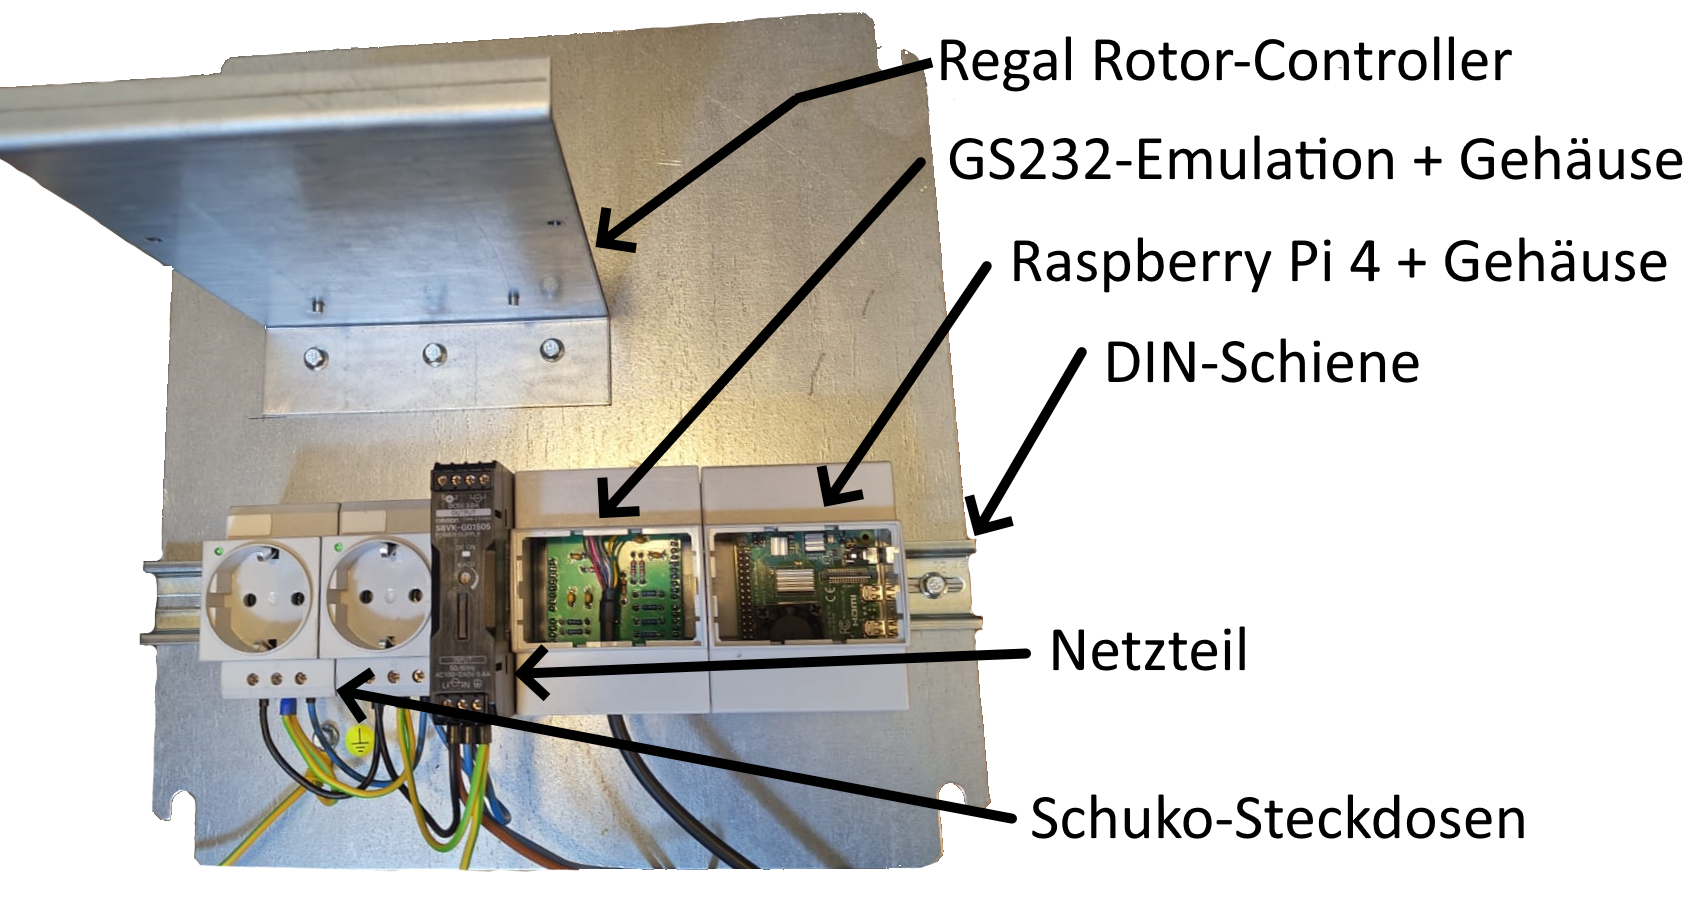
\includegraphics[width=0.7\linewidth]{../ref/Schaltschrank_Befestigung.jpg}
	\caption{Befestigungskonzept im Schaltschrank}
	\label{fig:schaltschrankbefestigung}
\end{figure}

\subsection{Anschlüsse am Schaltschrank}
Der Schaltschrank verfügt an der Außenseite über keinerlei Anschlüsse. Die Kabel für die Stromversorgung, Antenne und Rotoren verlaufen über Kabelverschraubungen nach außen um dort direkt verwendet werden zu können. 

\begin{figure}[H]
	\centering
	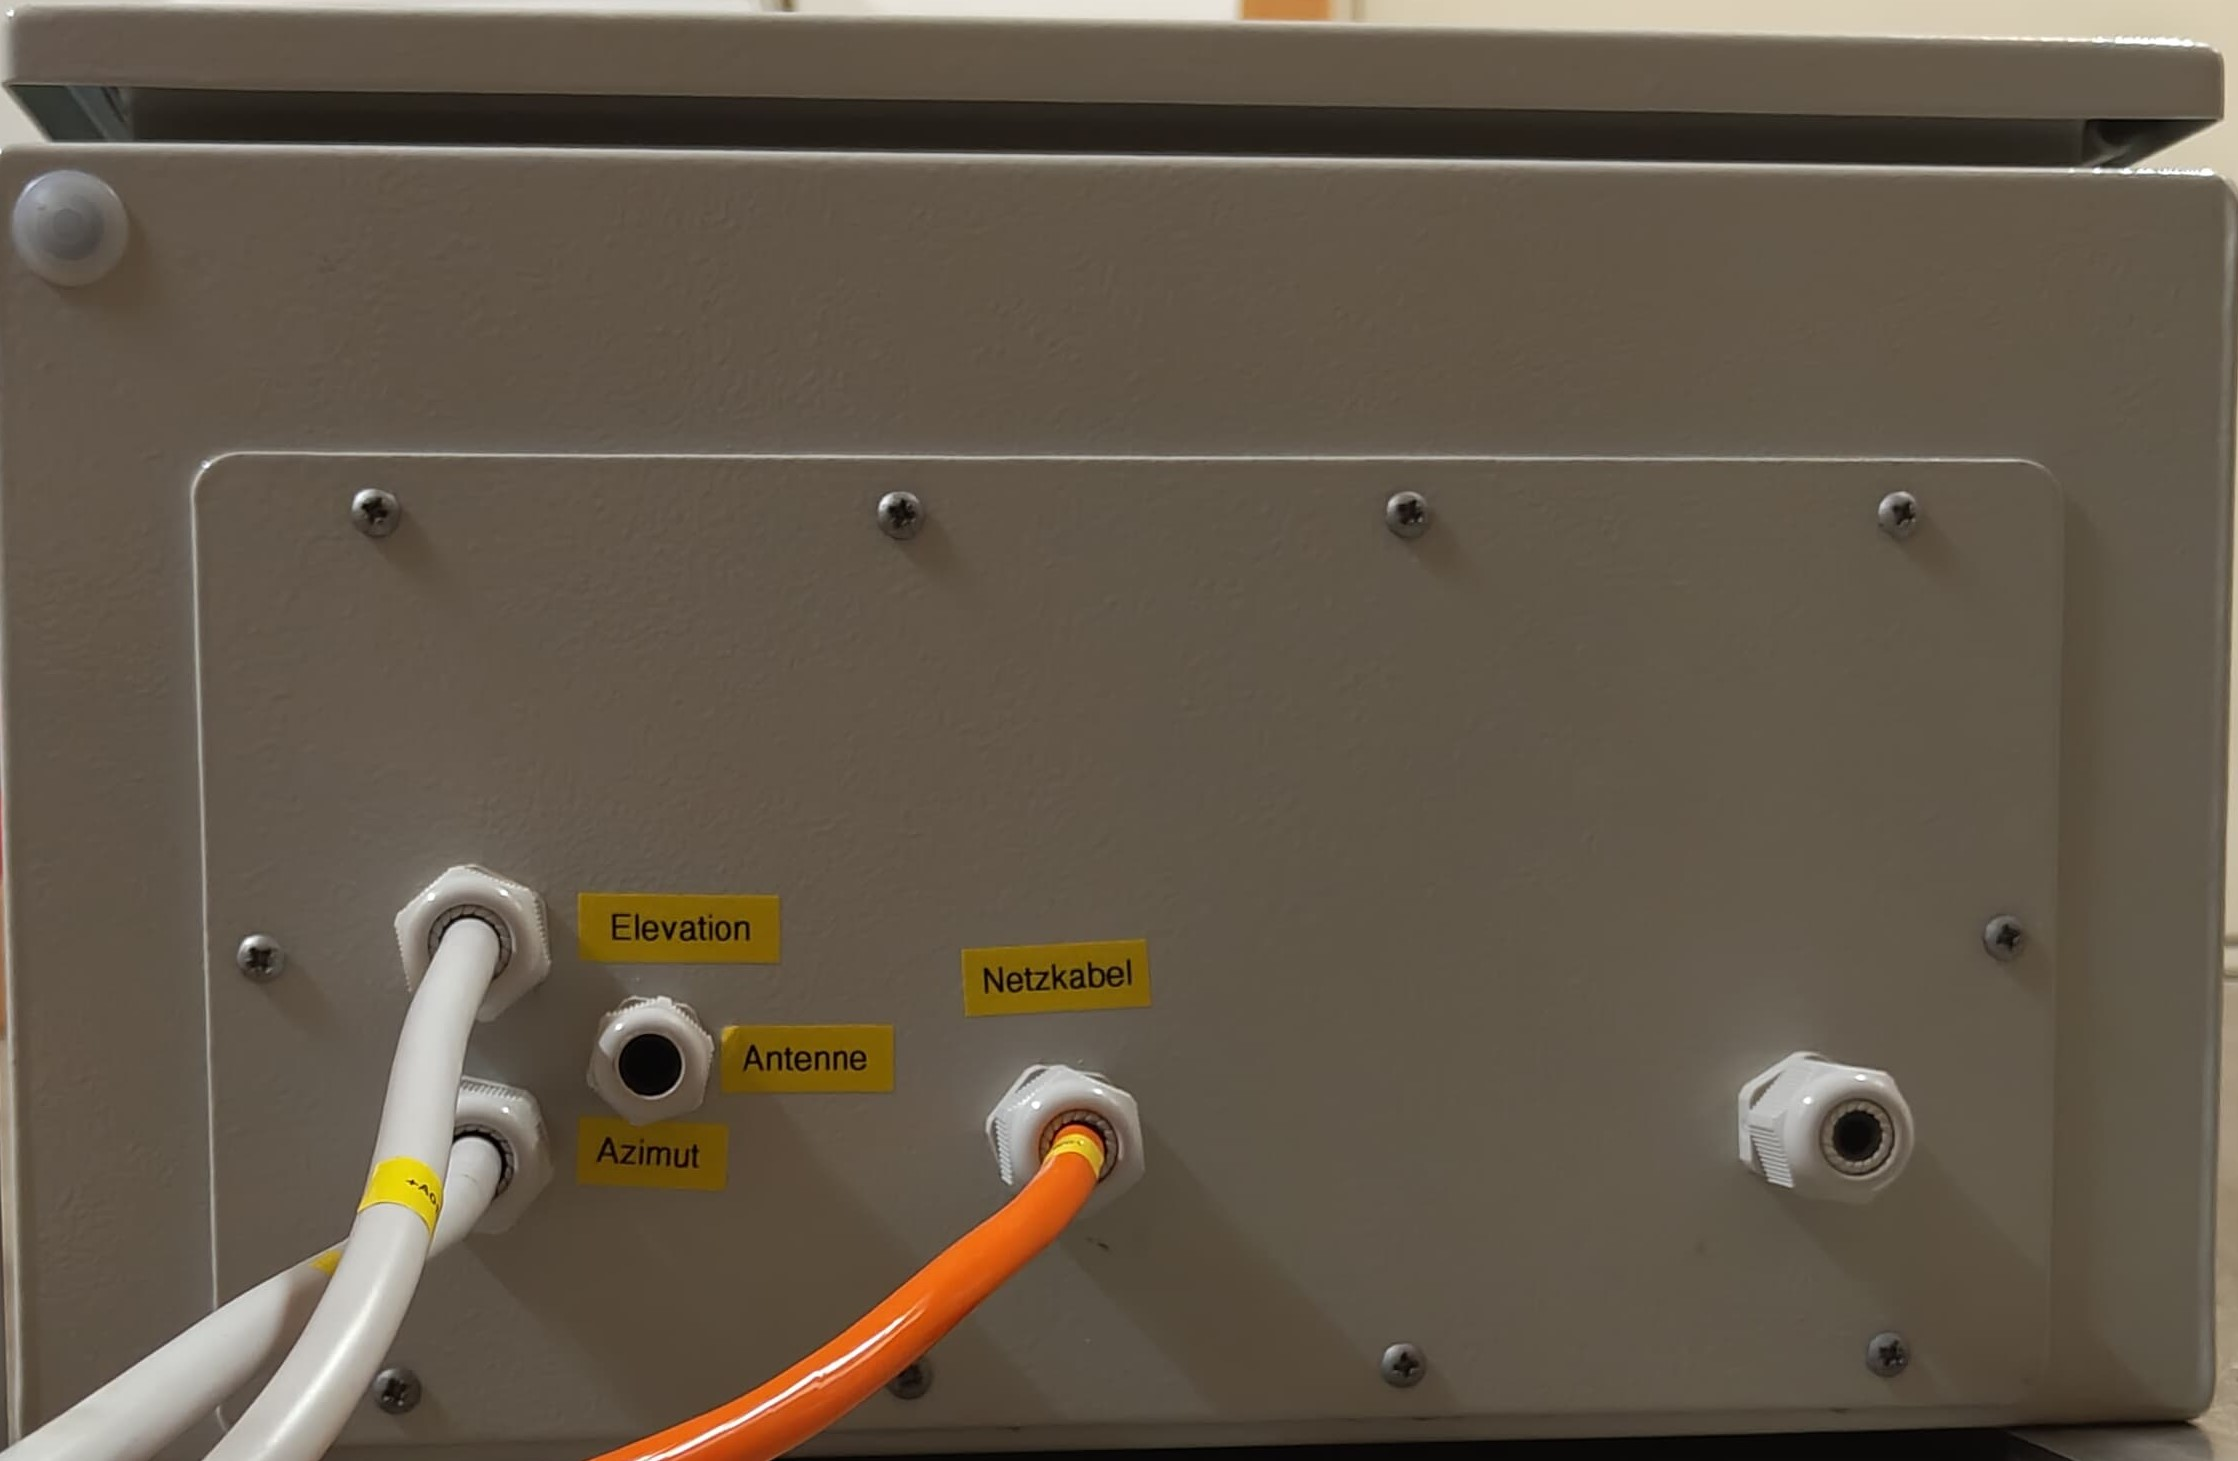
\includegraphics[width=0.7\linewidth]{../ref/Schaltschrank_Anschluss.jpeg}
	\caption{Anschlüsse am Schaltschrank}
	\label{fig:schaltschrankanschluesse}
\end{figure}

Die unbeschriftete Schraubverbindung in der Abbildung dient als Reserve für mögliche Erweiterungen.

\subsection{Standfüße}
Um den Schaltschrank flexibel platzieren zu können wurden zwei Standfüße aus 8 Millimeter Eisenblech zusammengeschweißt und mit Gummifüßen versehen. 

\begin{figure}[H]
	\centering
	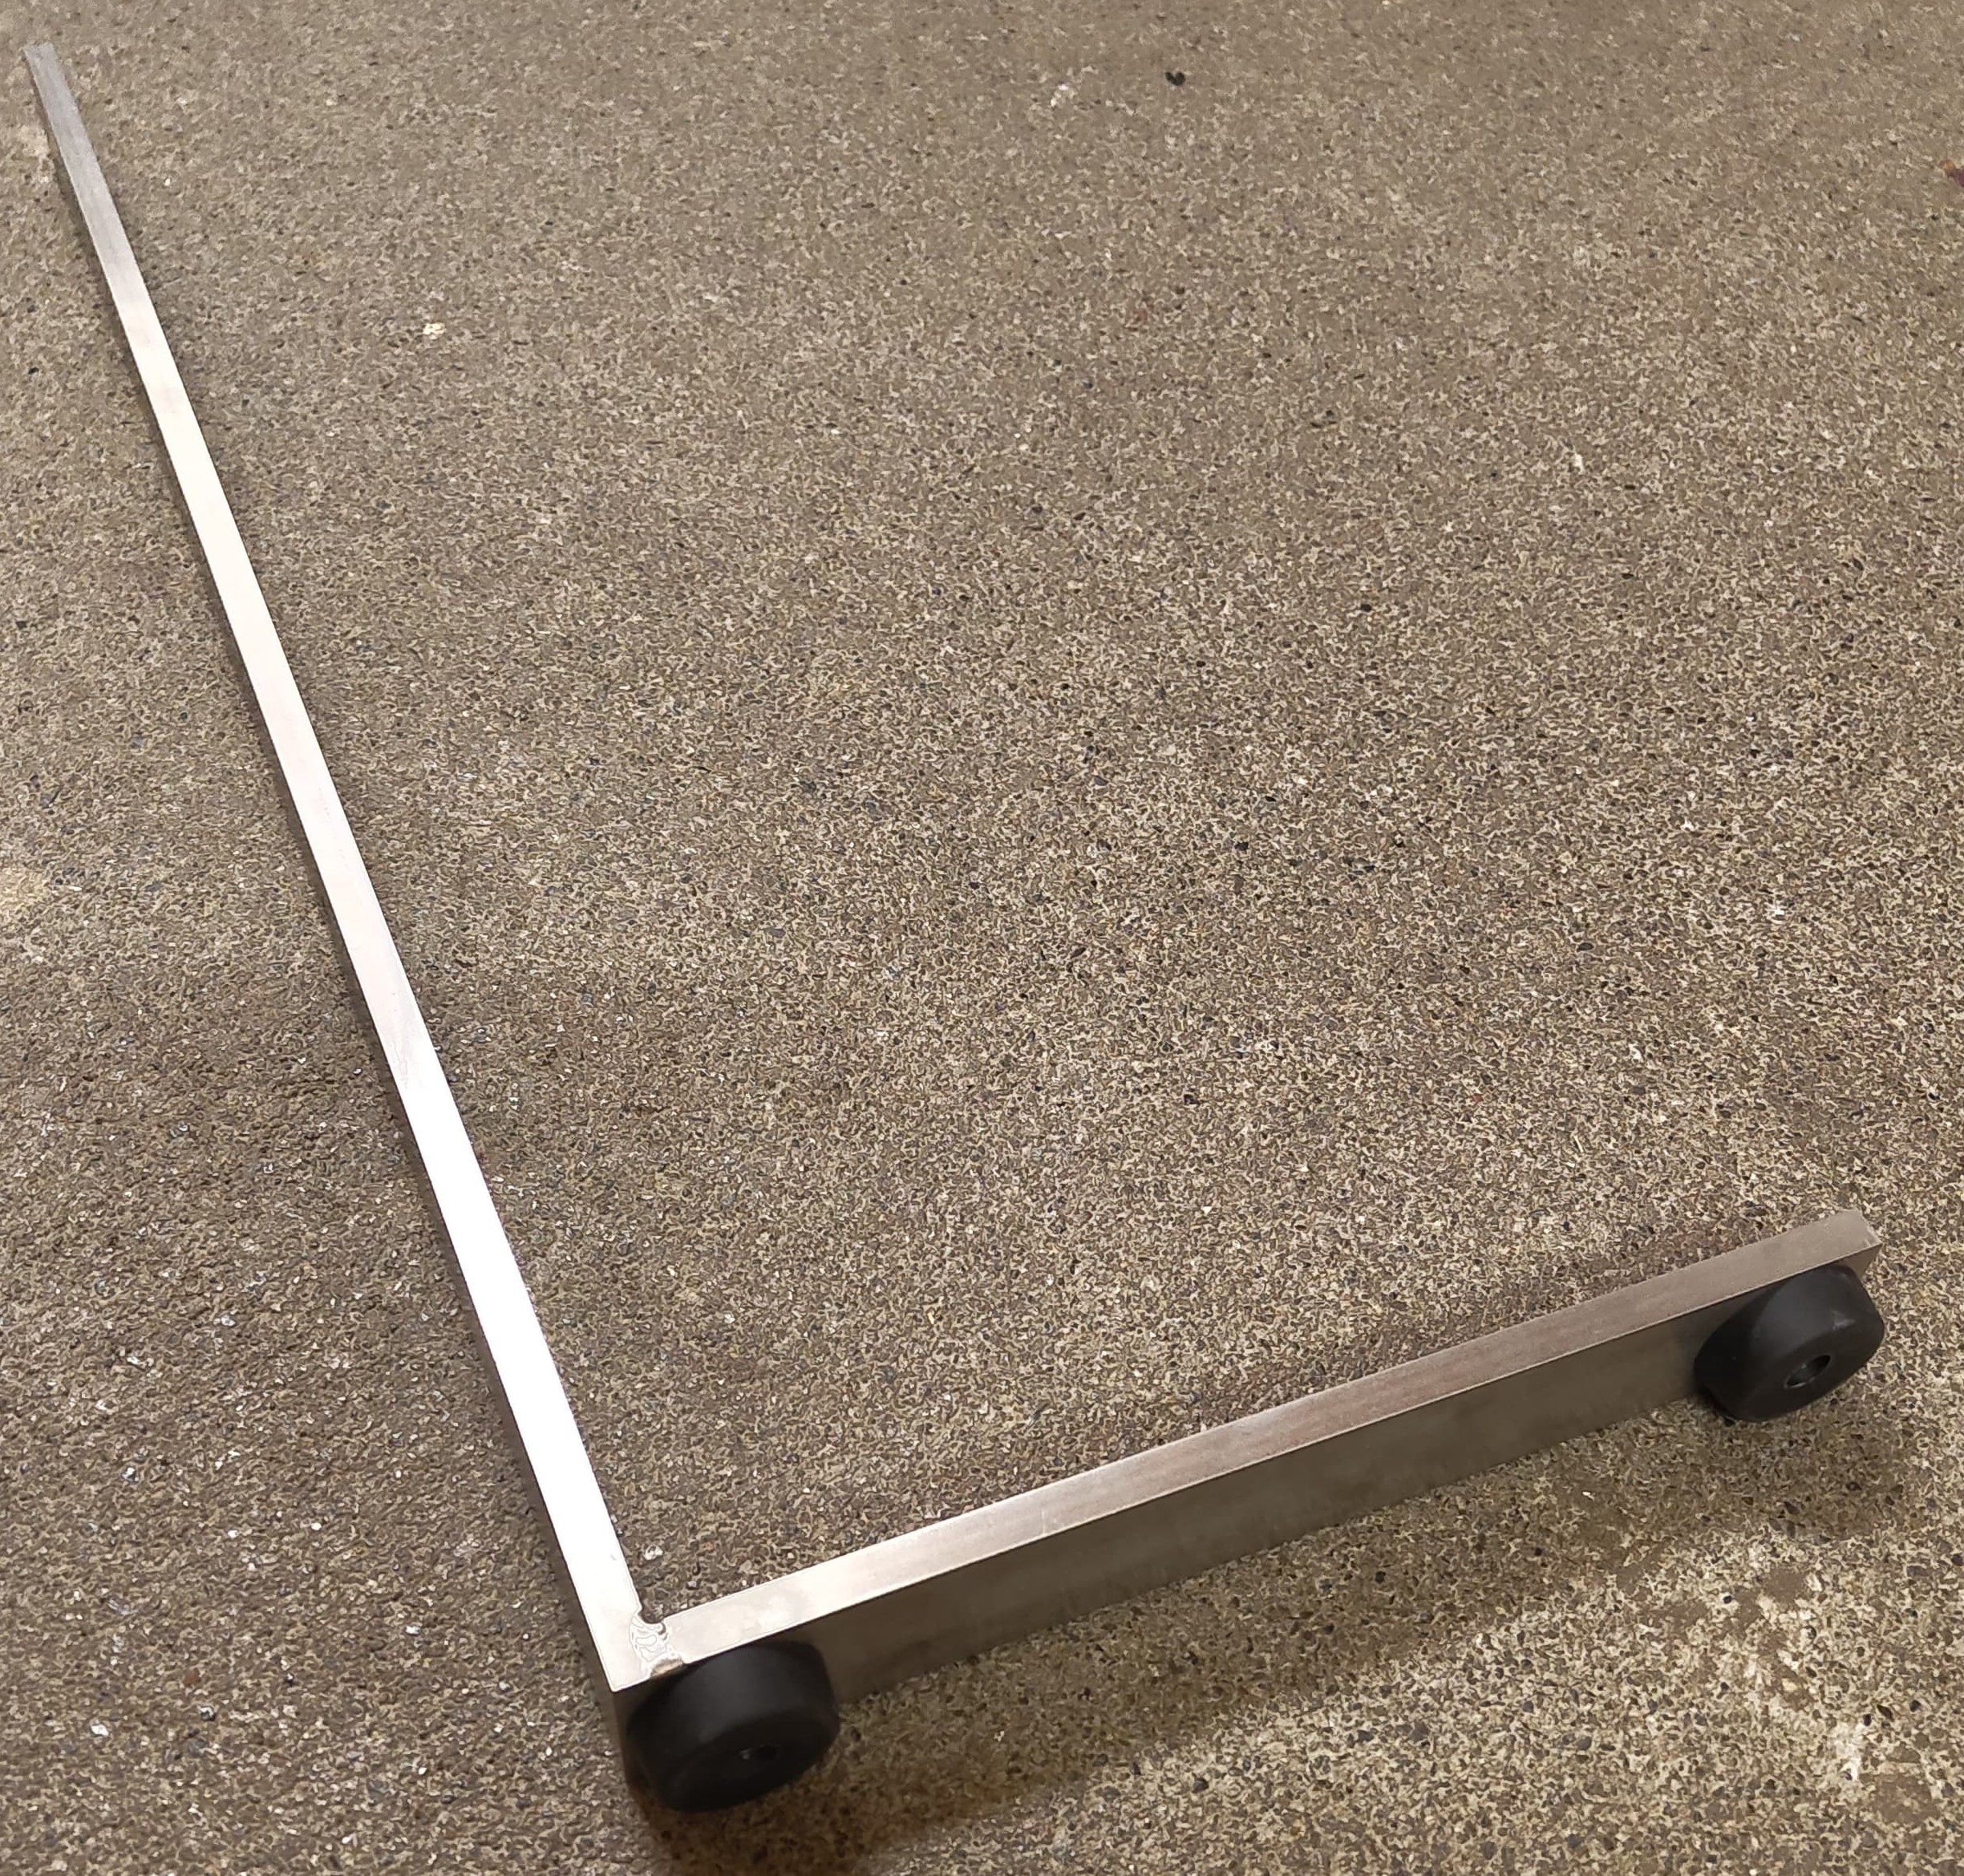
\includegraphics[width=9cm]{../ref/Schaltschrank_Fuss.jpeg}
	\caption{Standfuß für den Schaltschrank}
	\label{fig:schaltschrankfuss}
\end{figure}

Das Ergebnis ist ein modular platzierbarer und vielseitiger Schaltschrank:

\begin{figure}[H]
	\begin{minipage}[b]{.4\linewidth}
		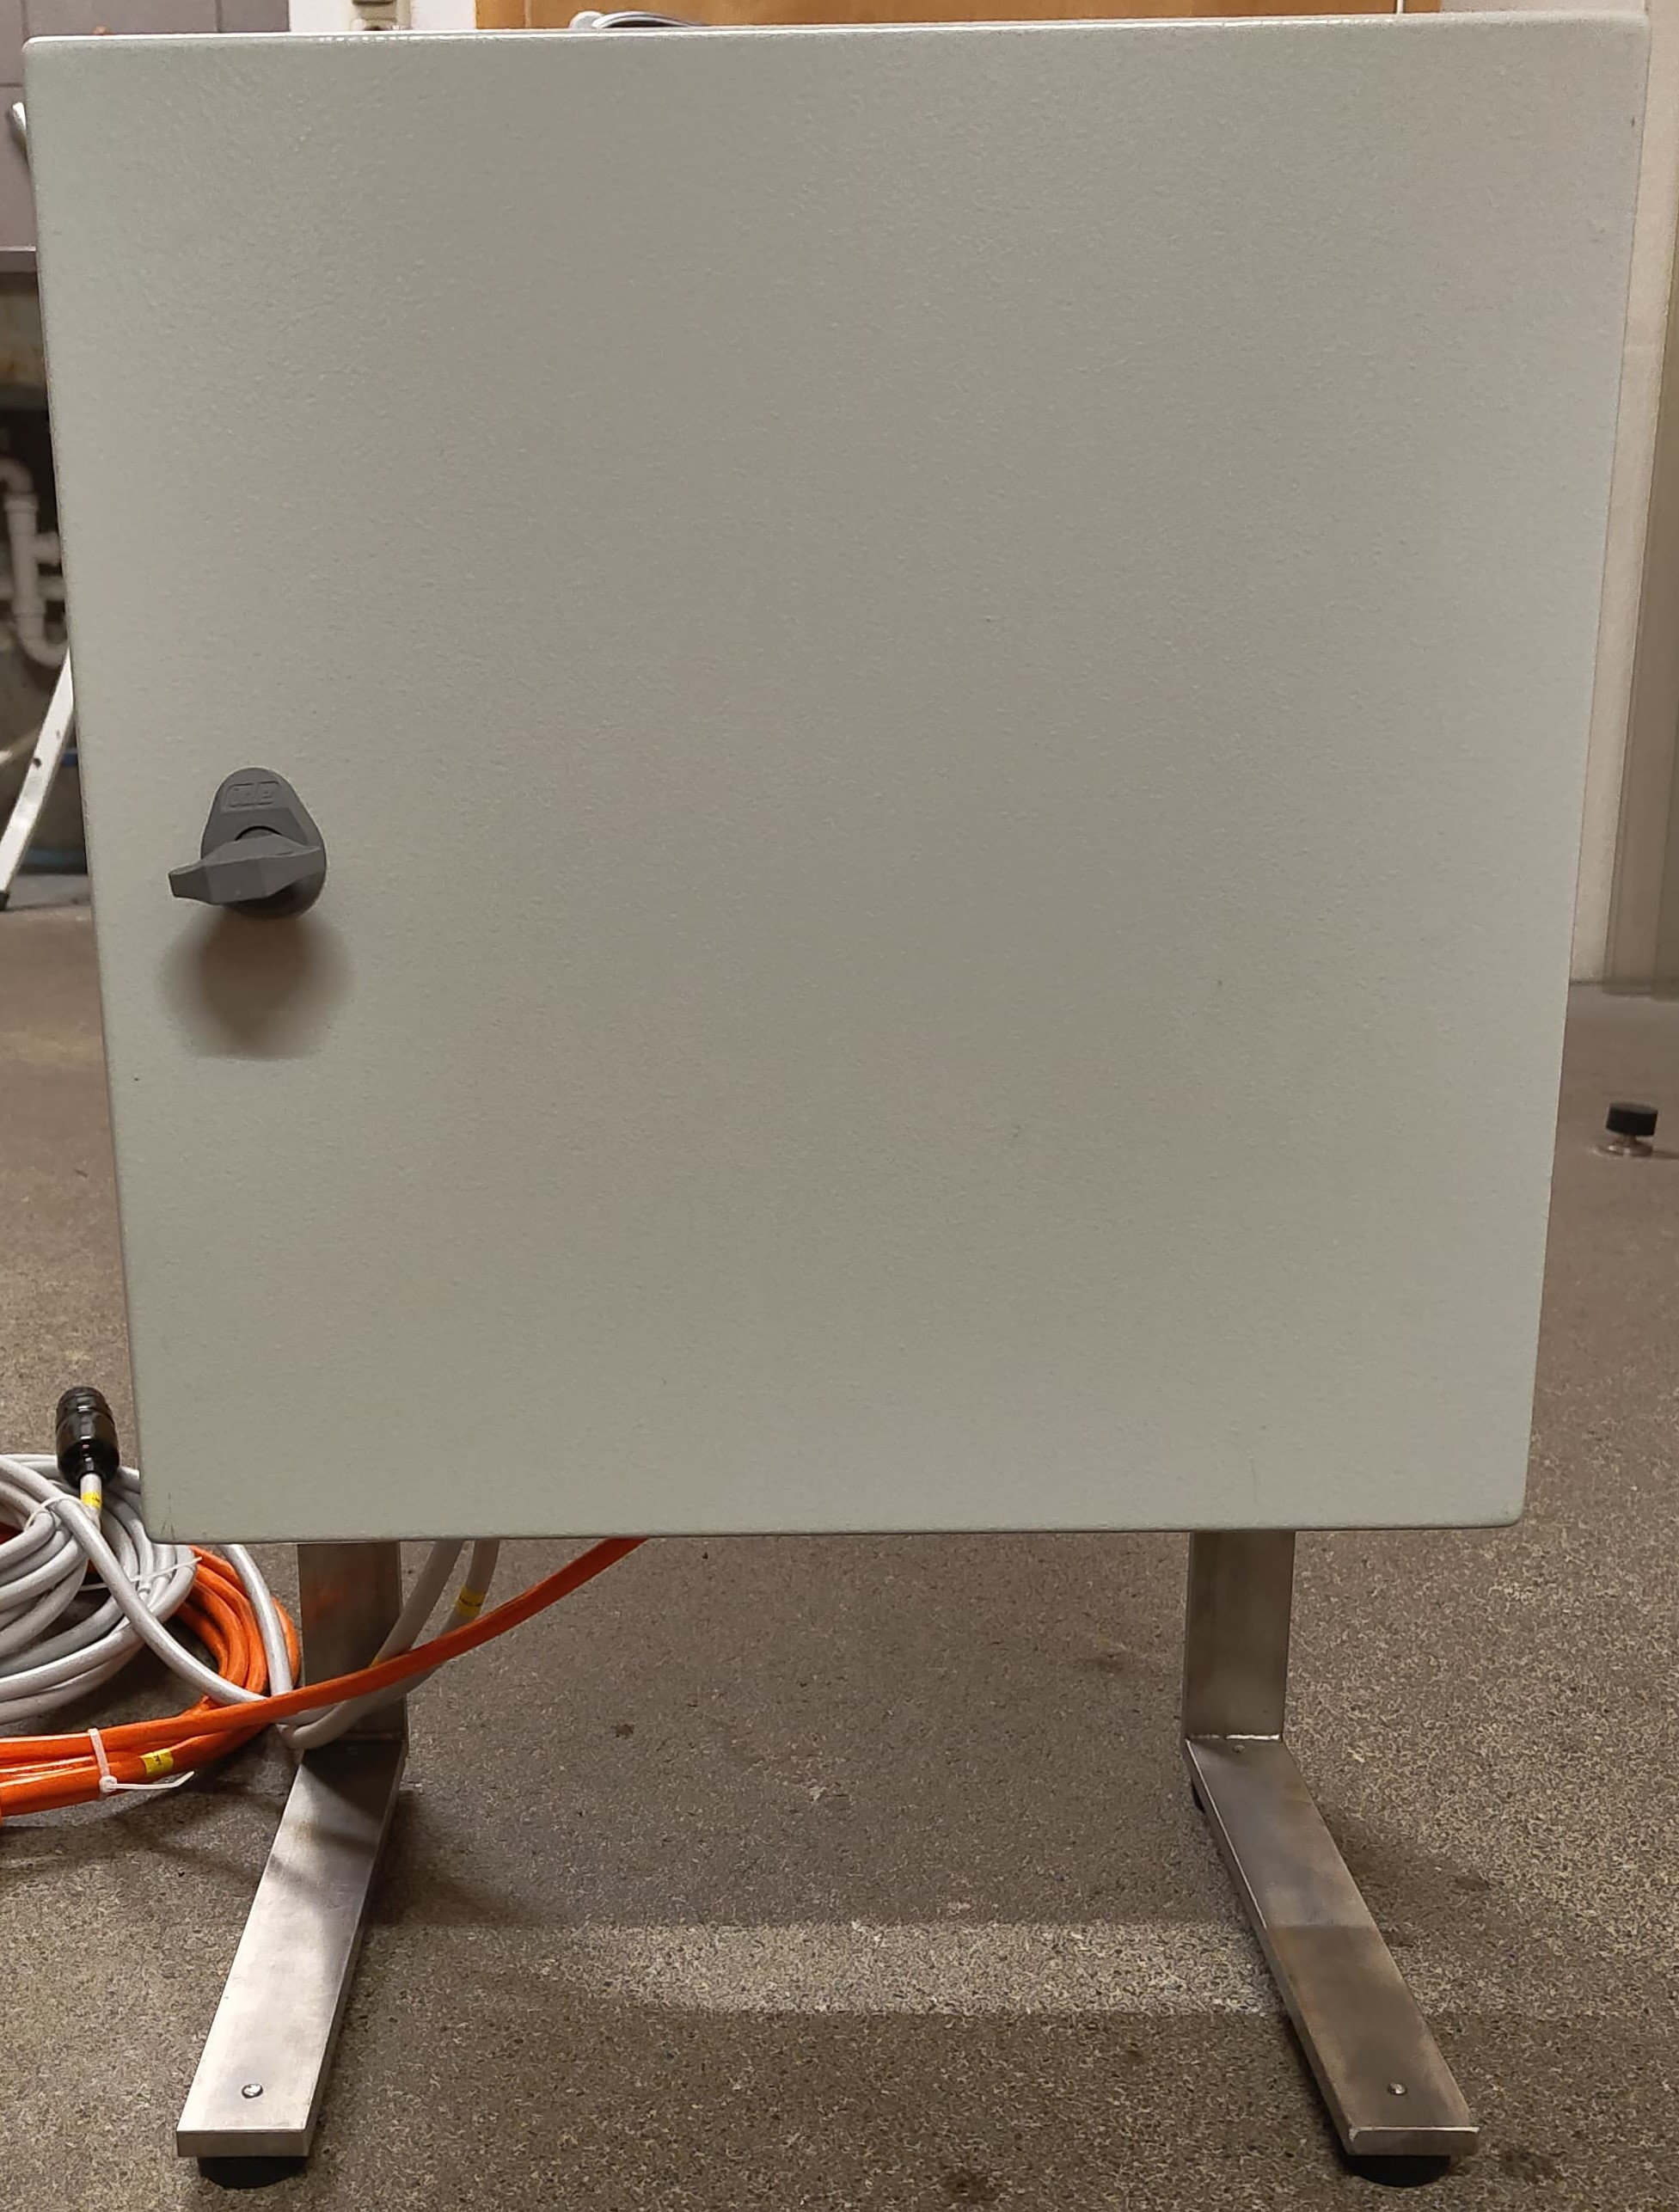
\includegraphics[width=\linewidth]{../ref/Schaltschrank_stehend_vorne.jpeg}
		\label{fig:schaltschrankstehendvorne}
		\caption{Schaltschrank stehend (Ansicht vorne)}
	\end{minipage}
	\hspace{.1\linewidth}% Abstand zwischen Bilder
	\begin{minipage}[b]{.4\linewidth} % [b] => Ausrichtung an \caption
		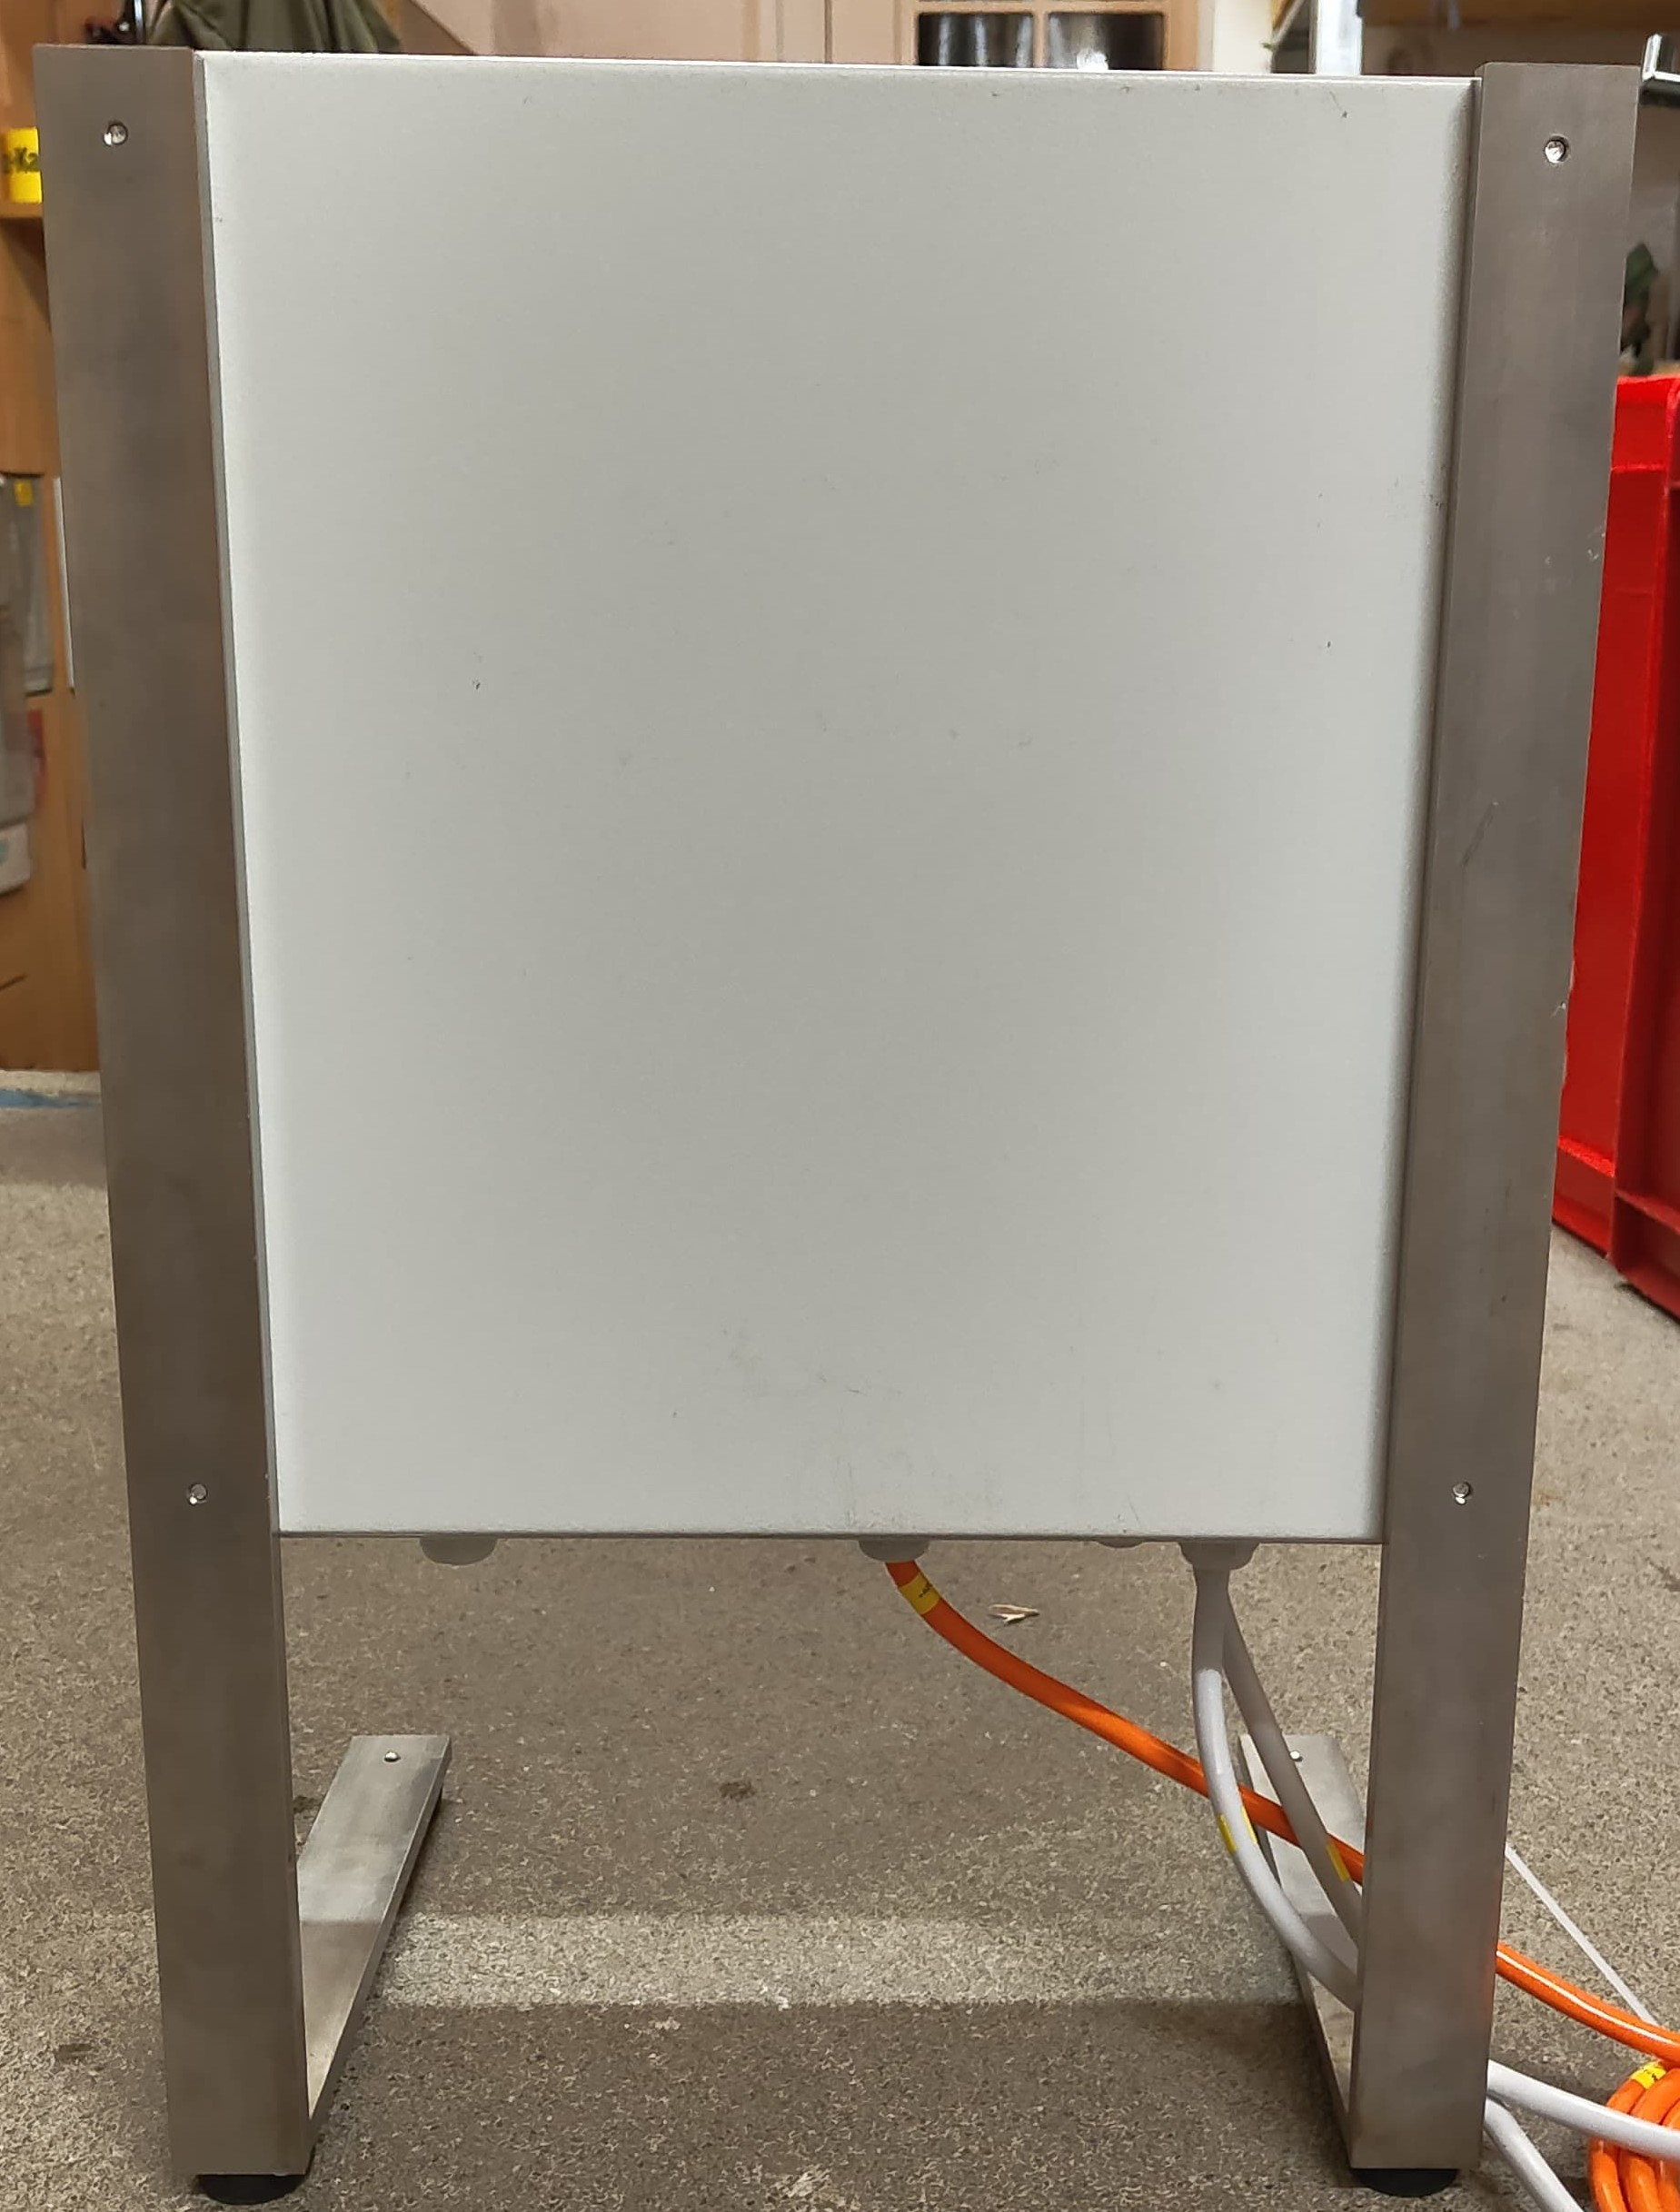
\includegraphics[width=\linewidth]{../ref/Schaltschrank_stehend_hinten.jpeg}
		\label{fig:schaltschrankstehendhinten}
		\caption{Schaltschrank stehend (Ansicht hinten)}
	\end{minipage}
\end{figure}




